\documentclass[11pt]{article}
\usepackage{/Users/mz/Box/repository/LaTeX/article}

\begin{document}
\section*{Extension}
\subsection*{Does Education Matter?}
RT ran analyses on various groups but surprisingly, they did not include education into account. One’s educational level, firstly, influences how s/he perceives the gun control problem directly. For instance, better-educated people are likely to have a better knowledge of the Second Amendment and therefore, have a different gun right attitude than others. Second, education also enables people to receive and process more information. Educated people are also expected to be more attentive to what is happening in the world. That said, education makes respondents more likely to receive the treatment. Third, education helps people to be more open-minded. RT argued the null effect of the Sandy Hook shooting is a result of the opinion polarization –– gun control opponents are frozen at their predisposition and reluctant to change according to the new information. We expect better-educated people are less change reluctance-prone. 

Education in TAPS wave 13 is measured in a 15-points scale, in which 1 means no formal education at all and 15 means doctorate. The 25\% quantile, median, and 75\% quantile is some college without a degree, an associate degree, and a bachelor degree respectively. 10 respondents refused to disclose their educational information. These invalid cases are only 0.6\% of the full sample so we simply drop them from our analysis. Since education has 15 categories, we treat is as a continuous variable. We include the treatment dummy variable, education, and their interaction term in our model to see whether the Sandy Hook shooting’s effect on gun control support is present conditional on one’s educational level. In the both models, we can write the independent variables and their coefficients (omitting the constant and cut points) as \(\beta_1\times t_i + \beta_2\times \text{education}_i + \beta_3\times t_i\times\text{education}_i\). Then, we clearly see \(\frac{\partial}{\partial t} = \beta_1 + \beta_3\times \text{education}\) gives use the effect direction.

In (), the term education itself is positive statistically significant at the \(\alpha = 0.001\) level in two models, demonstrating without the shooting, education increases a person’s support to gun control. However, when it comes to the conditional relationship of interest, neither the term \(t\) nor the interaction term shows statistical significance. Although it is incorrect to see conditional effect’s significance solely according to that of a single term, the lack of significance in both terms suggest regardless of a person’s education level, the Sandy Hook shooting does not change her/his support to gun control. 


\begin{table}
\caption{Effect of the Sandy Hook Shooting on Gun Control Support Conditional on Education}
\begin{center}
\begin{tabular}{l D{.}{.}{4.5} D{.}{.}{5.5}}
\toprule
 & \multicolumn{1}{c}{Logit} & \multicolumn{1}{c}{Ordered Logit} \\
\midrule
Post-shooting (Yes = 1)            & -0.50       & -0.09      \\
                                   & (0.78)      & (0.57)     \\
Education (No = 1, Doctorate = 15) & 0.17^{***}  & 0.12^{***} \\
                                   & (0.04)      & (0.03)     \\
Post-shooting \(\times\) Education & 0.05        & 0.03       \\
                                   & (0.07)      & (0.05)     \\
Constant                           & -3.07^{***} &            \\
                                   & (0.46)      &            \\
\(\tau,\) 1\textbar 2              &             & 0.90^{**}  \\
                                   &             & (0.34)     \\
\(\tau,\) 2\textbar 3              &             & 1.91^{***} \\
                                   &             & (0.35)     \\
\(\tau,\) 3\textbar 4              &             & 2.59^{***} \\
                                   &             & (0.35)     \\
\(\tau,\) 4\textbar 5              &             & 3.47^{***} \\
                                   &             & (0.35)     \\
\midrule
BIC                                & 1842.03     & 5041.52    \\
\(\ln\mathcal{L}\)                 & -906.17     & -2494.78   \\
\(N\)                              & 1674        & 1674       \\
\bottomrule
\multicolumn{3}{l}{\scriptsize{\(\tau\) denotes cut point. Standard errors in parentheses. $^{***}p<0.001$; $^{**}p<0.01$; $^{*}p<0.05$.}}
\end{tabular}
\label{tab2}
\end{center}
\end{table}


\section*{Extension Using New Data}
The null results reported in RT remain unchanged through our robustness replication. Could the null finding be driven by any inappropriate empirical operationalization? We argue RT’s measurement to the dependent variable deviates not only the Sandy Hook shooting’s context but also the intensive debate of the gun control issue in the US. Although the Sandy Hook shooter possessed a handgun, his assault-style semi-automatic rifle, accompanied with high-capacity magazines, is the primary weapon he used. Beyond the exact case context, the gun control debate in the US is more intensive around the restriction on assault weapons. In contrary, RT used the question which asks the support to banning the handgun possession, which goes too far for many people in the US context. From (), we see the pre-shooting support to banning handgun is even below 24\%, showing the handgun ownership ban goes too far for the vast majority of American people. Thus, we expect to see if the shooting event’s effect exists when the dependent variable is better measured.

Even the null finding drawn from a single case, i.e., the Sandy Hook shooting, reflect the true relationship, whether it is externally valid is still a natural concern. Therefore, we extend RT’s research by using another mass shooting event and a new survey question to measure the dependent variable. We select the 2016 Orlando nightclub shooting, which resulted 49 people killed and 53 wounded, for our extended study. Our selection criteria are based on the three following points. First, both the Sandy Hook and the Orlando shooting happened in presidential election year (2012 and 2016 respectively) so we are able to hold the general political context (e.g., debate intensity, opinion polarization, etc.) largely constant. Doing so make sure the result discrepancy (if any) is not a product of the general trend. Second, by the time of happening, the Orlando shooting was the most deadliest one in the US history. Its scale and impact make it the best candidate to evaluate the effect which was previously shown null. Third, the Orlando shooting happened on the 12\textsuperscript{nd}. This mid-month occurrence date naturally divides the respondents to two roughly equal-sized groups, avoiding the sample size imbalance between the treatment and control group.\footnote{Due to this reason, we do not select the 2017 Las Vegas shooting which happened on the 1\textsuperscript{st} October.}

We use the wave 55 data from TAPS to carry out our extension.\footnote{As we do in the robustness replication, we only focus on the cross-sectional sample here.} The respondents whose recorded questionnaire finish time was before the 12\textsuperscript{nd} June 2016 was coded as \(t_i = 0\), which means the pre-shooting (control) group. Those who answered the questionnaire after the 12\textsuperscript{nd} June (exclusive) are coded as \(t_i = 1\), which means the post-shooting (treatment) group. After the data cleaning which will be briefly described below, the valid cases in the sample are 1581. Among them, (). For the dependent variable, we use the following question (the code in TAPS’ data manual and dataset is \texttt{ISSUESA4GS55}): 
\begin{displayquote}
\itshape
Do you generally support or oppose gun control legislation?
\end{displayquote}
The meaningful response to this question is binary | oppose (coded as 0) and support (coded as 1). In the sample, only 1\% respondents refused to answer this question and we drop them from our analysis. A potential problem comes from the no opinion answer, which was chosen by 7\% of the respondents. The first concern is the binary nature of the allowed meaningful answer in this question may coerce some in-between respondents (who would give a neither or neutral answer when applicable) to this category. Also, regarding an issue which is related to the vital public interest like gun control, no opinion is also a sort of opinion to some degree. In other words, they also expressed some substantively meaningful thoughts through a seemingly meaningless answer. However, since our primary interest in this research is evaluating an exogenous event’s marginal effect on gun control, instead of comprehensively explain its variation among different people, we argue dropping the no opinion observations does not harm the principal target of our analysis. Nevertheless, if the second concern were present, then our results would be biased. This concern is the no opinion answer is not randomly allocated among the two groups and instead, one group has a disproportionately higher number of no opinion respondents. If this was the case, then we would have dependent variable’s missingness conditional on the treatment variable. To rule out this possibility, we regress a binary variable indicating whether a respondent has an opinion (answering oppose or support) or not (answering no opinion) on the treatment variable \(t_i\) through a logit model to see if the treatment status predicts the respondents’ probability of giving an no opinion answer. The statistical insignificance of \(t_i\)’s coefficient suggests there is no evidence to support the claim that the no opinion answer rate is different between the treatment and control group. Therefore, we delete the cases of no opinion and keep our dependent variable in its binary nature. 

We follow RT’s regressions-on-sub-samples approach and apply logit model for estimation, which is as same as (). The included group indicators in our analysis are gender, parental status, ideology, Obama support, political interest, news consumption frequency, and political knowledge.\footnote{Other interesting group indicators, such as geographical proximity to the shooting location, are unfortunately unavailable in TAPS wave 55.} The first three are included in RT and common factors that are taken into account in investigating people’s gun control attitude. The questionnaire asks the respondents to self-identify themselves on a 6-points ideological scale in which the left is liberal and the right means conservative. We collapse this scale to a dummy variable in which 1-3 equals liberal and 4-6 equals conservative. Obama support is a proxy for the respondents’ partisanship since the latter is not directly asked in TAPS wave 55. We assume Democrats are more likely to support Obama while Republicans do the opposite. The question asks the extent which the respondents agree with Obama’s work.\footnote{Half of the observations are missing due to an undocumented reason for this question.} We classify strongly and somewhat agree into the support category. Strongly and somewhat agree, plus not sure, go to the non-support category. We include political interest, news consumption frequency, and political knowledge since all of them are correlated with the likelihood of a person’s attention to the Orlando shooting, in other words, the degree of compliance to the treatment. Specifically, we code very and somewhat interested in politics as having political interest and slightly and not at all interested in politics as not. For the news consumption frequency, we code everyday as 1 and all others as 0. This coding rule results two relatively balanced sub-samples. There is a battery of political knowledge questions in TAPS wave 55. Among them, we choose the one asks the US senator’s term. The coding is binary as well, in which the correct answer is one while all others (including don’t know) are 0. In our sample, surprisingly, only half American people gave the correct answer. We drop all refused answers but for the political knowledge question. The US senator’s term is an insensitive, neutral, and fairly short question so we hardly find a valid reason for refusing to answer it. In other words, we argue the respondents who know the answer would just give the correct answer while refusing means the respondent did not firmly possess the knowledge. Some variables in the list above are categorical but we collapse them all to dichotomous versions for the analysis simplicity. We believe for extending a null finding, it is better to start from relatively simple specifications. If the null finding is overrode, then we advance the analytical complexity to see whether the new finding holds. If the null finding does not change, then it suggests the null finding is robust.

As we do in our robustness replication, we calculate the predicted probabilities with the confidence intervals to visually show the results (). Across all panels, we see the confidence intervals for \(t_i = 0\) and that for \(t_i = 1\) are over-lapping, indicating there differences are not statistically distinguishable. Substantively, it means the Orlando shooting does not change American people’s gun control attitude irrespective of their personal characteristics. Our null results show American people, even after repeated bloody tragedies and intensive debates, are still unresponsive to the tragic mass shooting. Since the null finding is theoretically puzzling, we further investigate the possible channels it could happen. As we discuss earlier, compliance is an inevitable concern in our research setting. People forget things and there is no guarantee that the Orlando shooting was still actively present in the respondents’ cognitive activities when they answered the questionnaire two weeks later. Hence, we narrow the sample down to the respondents whose survey finish dates are even closer to the 12\textsuperscript{nd} June, the day of the Orlando shooting. Specifically, we restrict our sample to the respondents who answered the questionnaire within 3 days before the shooting and within 7 days after the shooting.\footnote{The imbalance between the pre- and post-shooting days happens because the respondents answered the questionnaire concentratedly before the 12\textsuperscript{nd} June.} Doing so gives us a new sample with \(N = 779\), in which (). However, the null results remain unchanged. From (), we see the predicted probabilities of gun control support are not statistically distinguishable between the two groups. It means even for the people who are more likely to comply with the treatment, the Orlando shooting still does not alter American people’s gun control support.
\begin{figure}[htbp!]
    \centering
    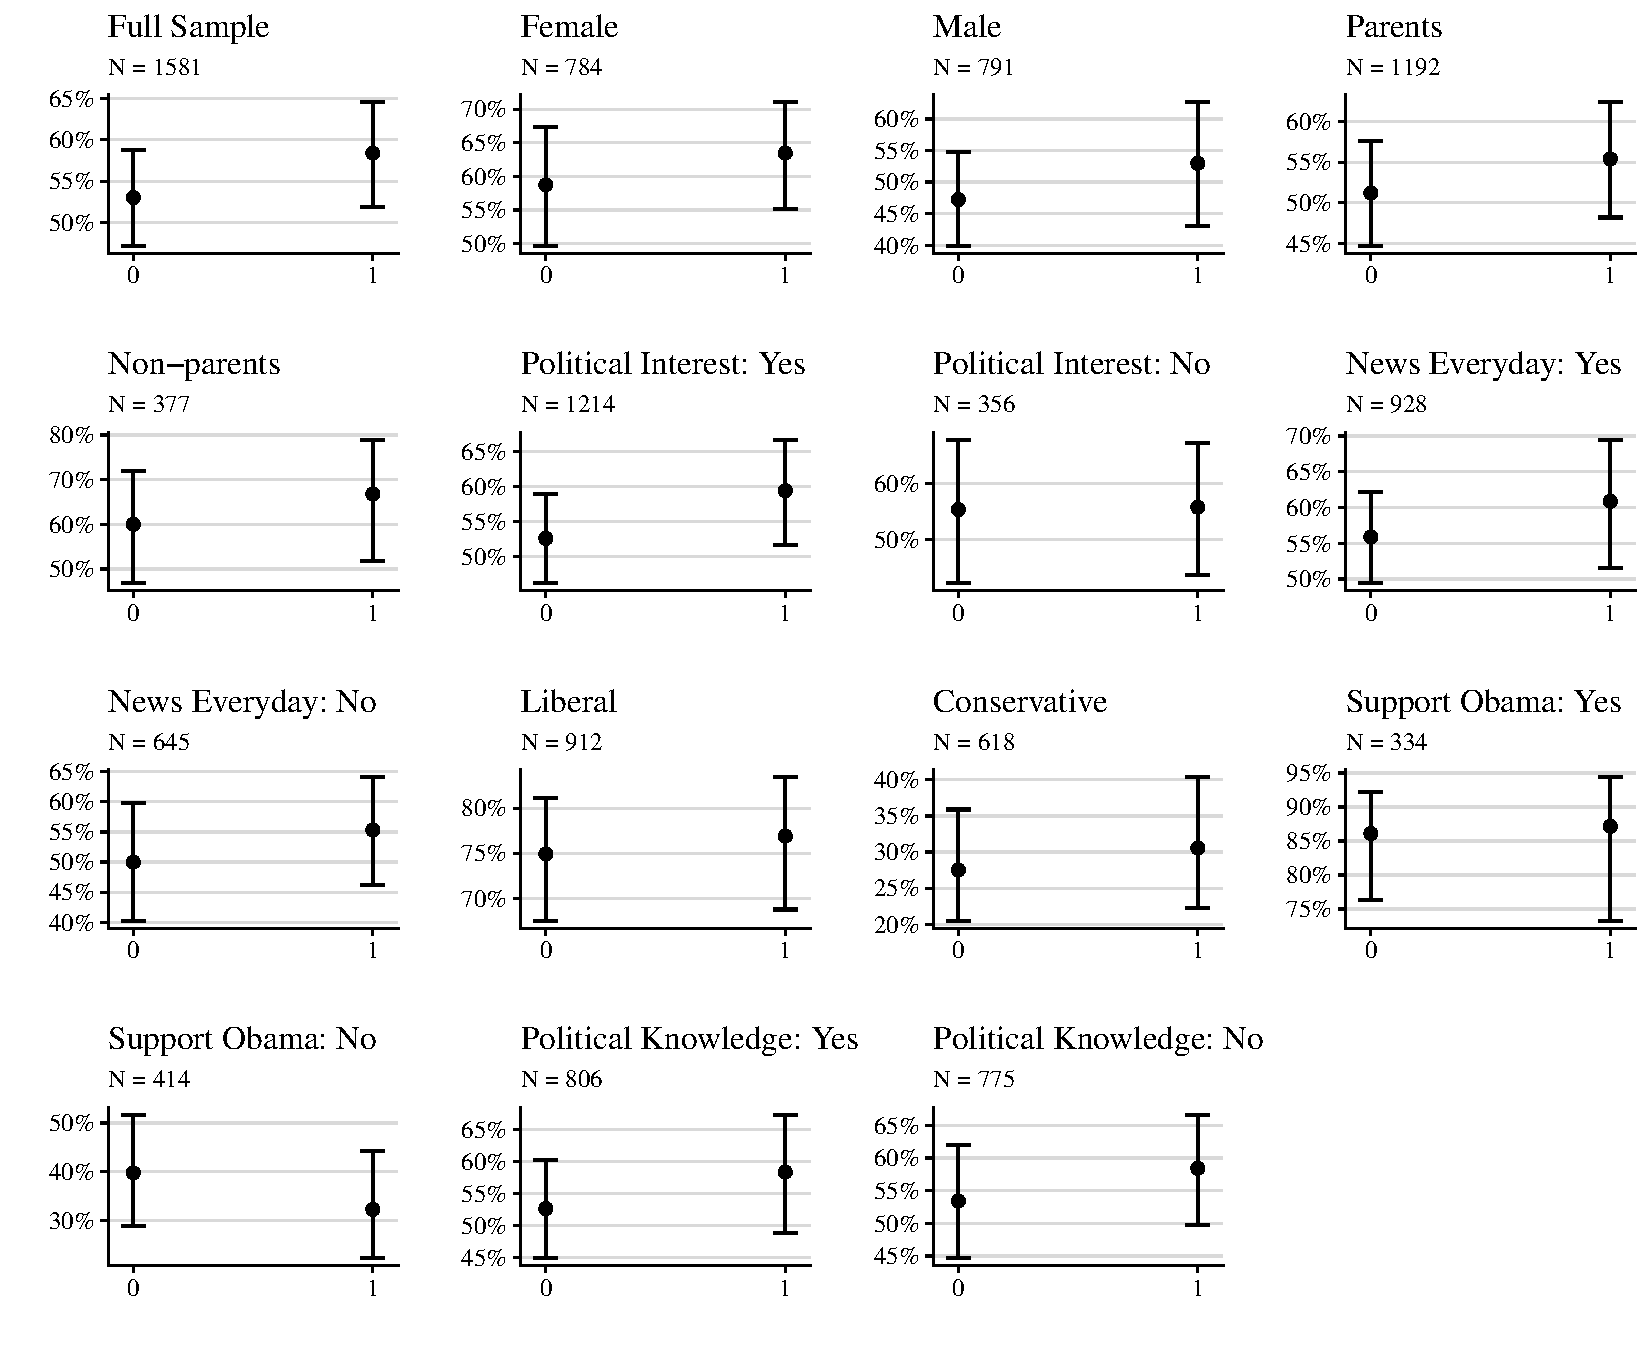
\includegraphics[width = 0.9\linewidth]{/Users/mz/Box/repository/replication/rogowski_tucker_2019_psrm/figs/fig2.pdf}
    \captionsetup{justification = raggedright, singlelinecheck = false}
    \caption{Predicted probabilities of gun control support before and after the 2016 Orlando shooting. In the \(x\)-axis, 0 means pre-shooting and 1 means post-shooting. The error bars show the 95\% confidence intervals, which are calculated by the Delta method.}\label{fig2}
\end{figure}
\begin{figure}[htbp!]
    \centering
    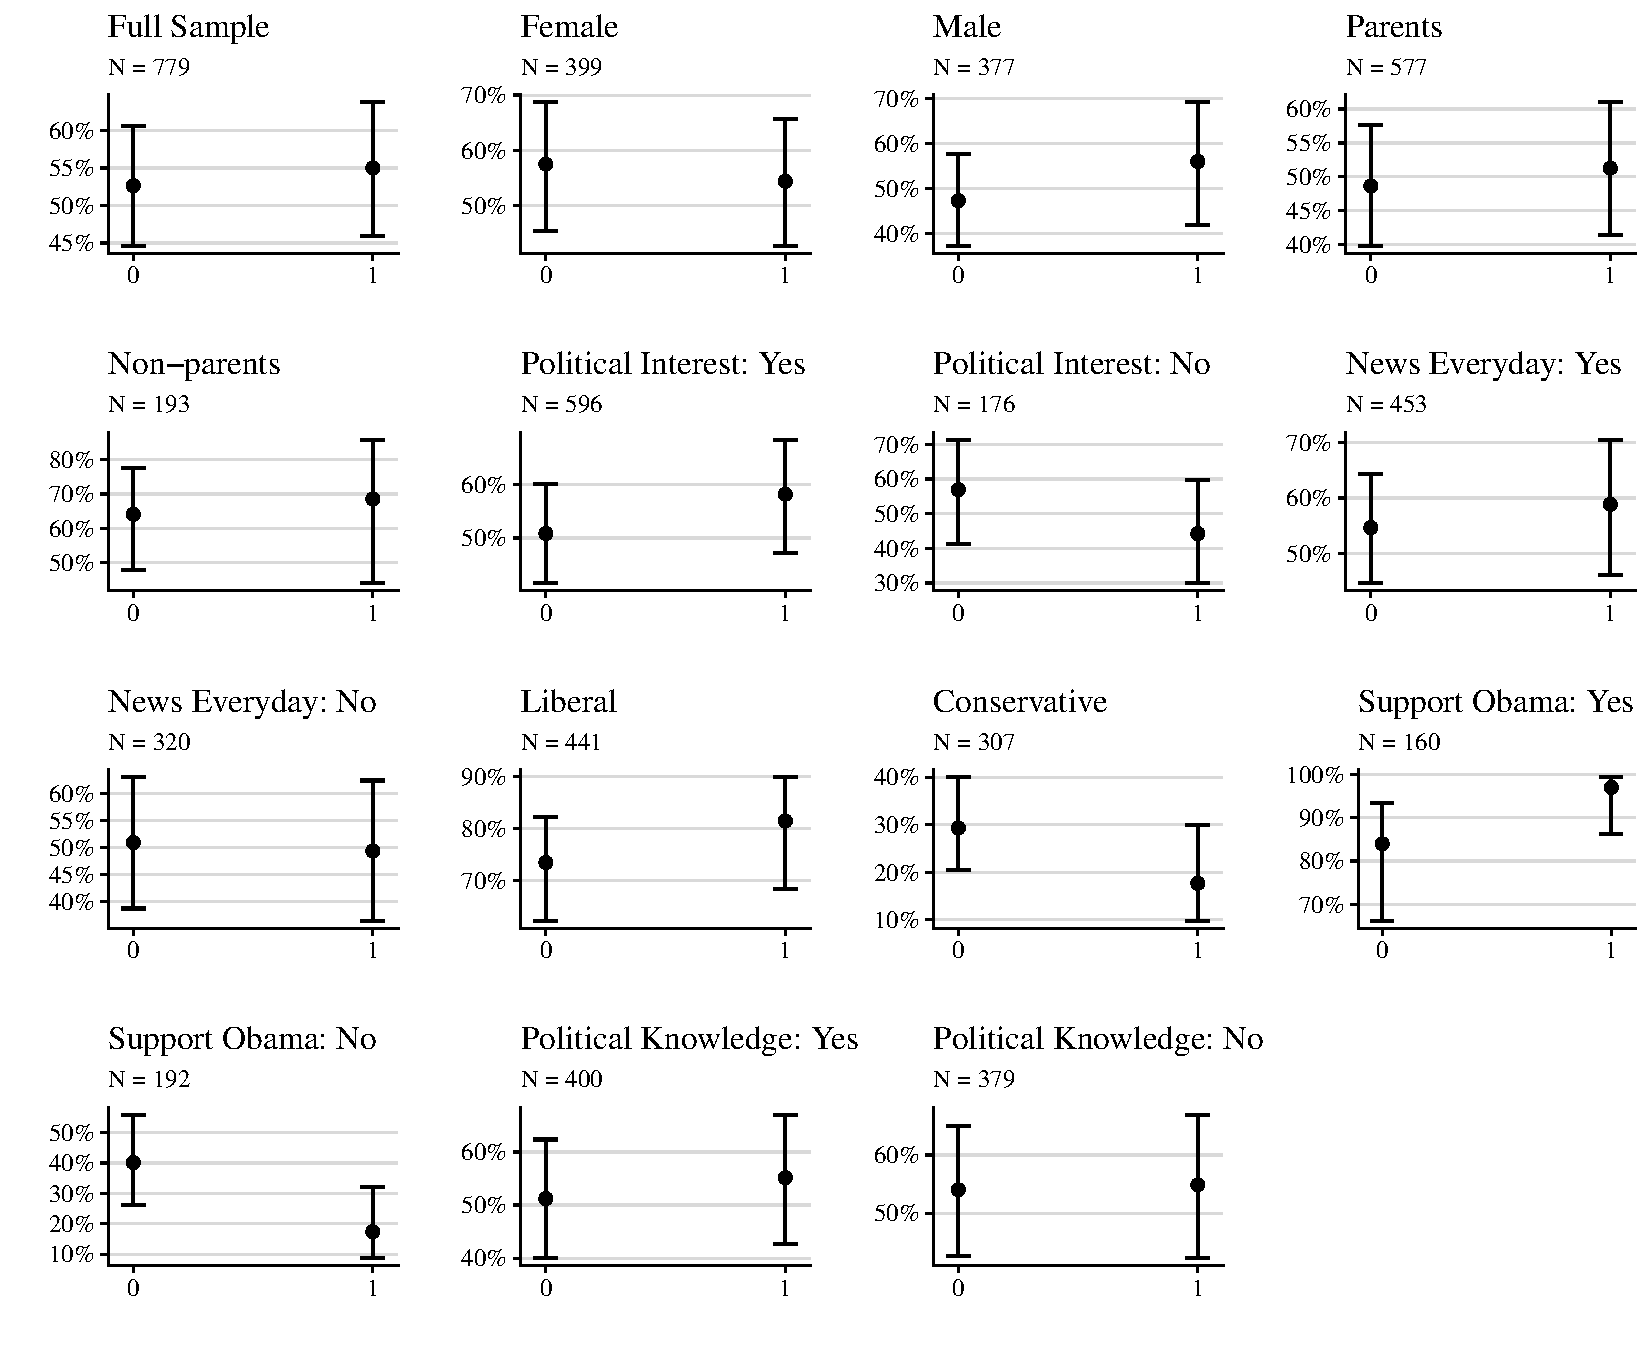
\includegraphics[width = 0.9\linewidth]{/Users/mz/Box/repository/replication/rogowski_tucker_2019_psrm/figs/fig3.pdf}
    \captionsetup{justification = raggedright, singlelinecheck = false}
    \caption{Predicted probabilities of gun control support before and after the 2016 Orlando shooting. The sample now only includes respondents who finished the survey within 3 days before and 7 days after the shooting. In the \(x\)-axis, 0 means pre-shooting and 1 means post-shooting. The error bars show the 95\% confidence intervals, which are calculated by the Delta method.}\label{fig3}
\end{figure}

\end{document}